\chapter{Metodologia}

Por conseguinte é natural a utilização de Redes Complexas como modelagem para estudos da Covid-19. Para tanto precisamos agora de dados sobre redes de contágio que contenham informações relevantes para esse estudo, como idade, tempo de contato, se faz parte de grupo de risco ou não, dentre outros.

Entretanto, não é fácil encontrar um banco de dados tão completo assim e não enviesado pela recente pandemia. Em 2008, visando o estudo da pandemia de influenza, a Comissão Europeia criou o projeto chamado POLYMOD \cite{POLYMOD} que tinha o intuito da coleta de dados para entender quais seriam os padrões de contatos da Europa \cite{Mossong2008}. Apoiado nesse estudo, pesquisas posteriores se inspiraram no molde do POLYMOD \cite{Belga2009,Belga2010,China,France,HongKong,Peru,Russia,Thailand,Vietnam,Zambia,Zimbabwe}.

\section{Análise dos Dados}

O foco dessa pesquisa será no banco de dados da França \cite{France} durante o primeiro semestre de 2012, ele foi coletado a partir de ligações aleatórias da população francesa excluindo territórios ultramarinos. Cada indivíduo que atendesse o telefone receberia um diário de contato para ser preenchido em 2 dias. Apenas uma pessoa por ligação poderia participar, com exceção de crianças e adolescentes para ter uma maior precisão e nesse caso um adulto ficaria responsável por fazer ou auxiliar. Ao final do dia a pessoa teria que preencher o diário anotando sobre informações pessoais, ambiente (escola, trabalho, casa,...) e as pessoas na qual teve contato de curto alcance no dia, a idade aproximada (ou exata) dessas pessoas, duração da conversa, frequência na qual têm contato, dentre outras informações, além disso para facilitar a memorização notificação os participantes foram instruídos a anotarem no máximo 40 contatos. Caso o participante fosse empregado, ele teria que informar qual a média de contatos no seu trabalho, caso fosse maior que 20 então os contatos que seriam anotados no diário seriam os não profissionais.

Toda a pesquisa era para acontecer em dois períodos: Fevereiro a Março e Abril a Maio de 2012. Contudo, no primeiro período foram recrutados menos pessoas do que deveriam e para corrigir isso foi criado um novo período em Abril para completar o primeiro. No total 24.250 pessoas receberam as ligações, 3.977 diários foram enviados, 2033 foram devolvidos e 2029 diários apresentaram contatos próximos. A Figura \ref{Idade_mes} mostra o número de contatos por dia em cada mês dos períodos da pesquisa.

\begin{figure}[H]
  \centering
  \captionsetup{font=normalsize,skip=1pt,singlelinecheck=on,labelsep=endash}

  \caption{Número de Contatos por mês}

  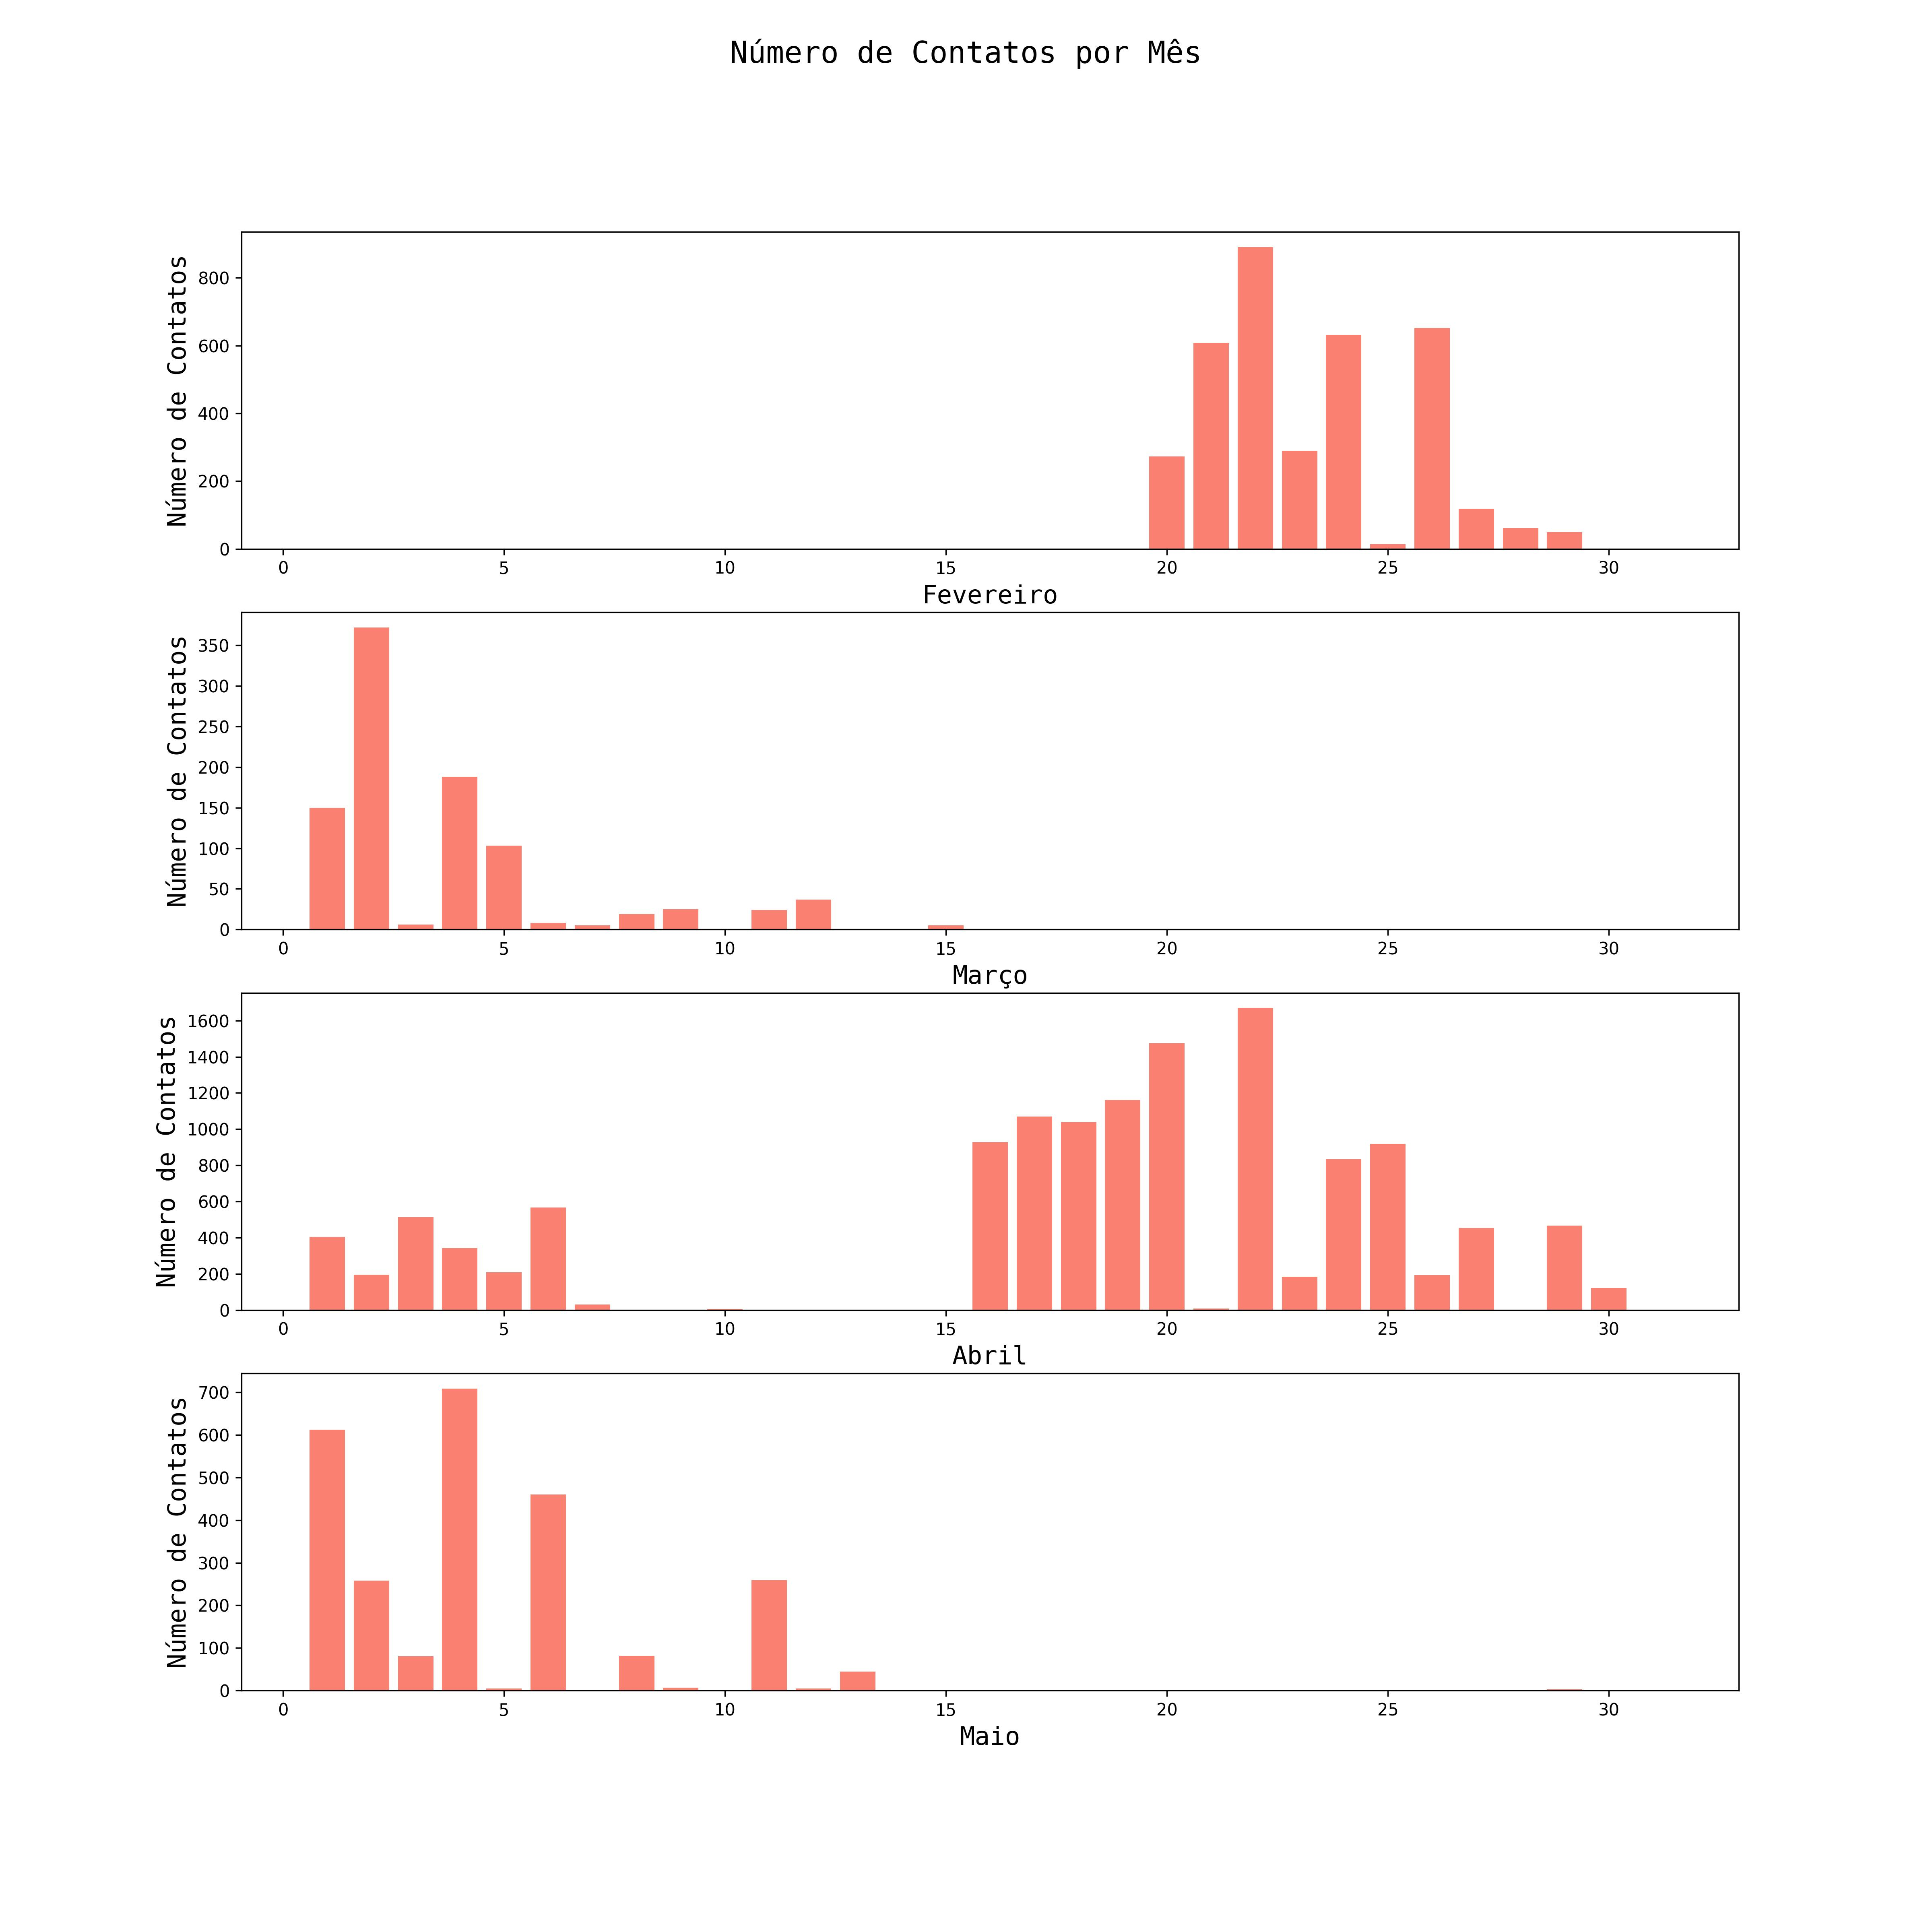
\includegraphics[scale=0.4]{./img/contatos_mes.jpg}
  \captionsetup{font=small,position=below,skip=-1pt}
   \caption*{\\Fonte: Autor.}
   \label{Idade_mes}
\end{figure}

A partir desses dados vamos coletar alguns resultados deles. Na Figura \ref{M_Idade} percebemos que a idade é um fator importante nos seus contatos. Nos primeiros anos de vida do ser humano seus contatos estão limitados a ficar dentro do seu convívio familiar, com o passar dos anos ele consegue ter maior liberdade para sair de casa e ter mais contatos com indivíduos, mas ao chegar no final da vida, depende-se cada vez mais do contato familiar pela limitação da idade.

\begin{figure}[H]
  \centering
  \captionsetup{font=normalsize,skip=1pt,singlelinecheck=on,labelsep=endash}

  \caption{Gráfico do Número de Contatos por Idade}

  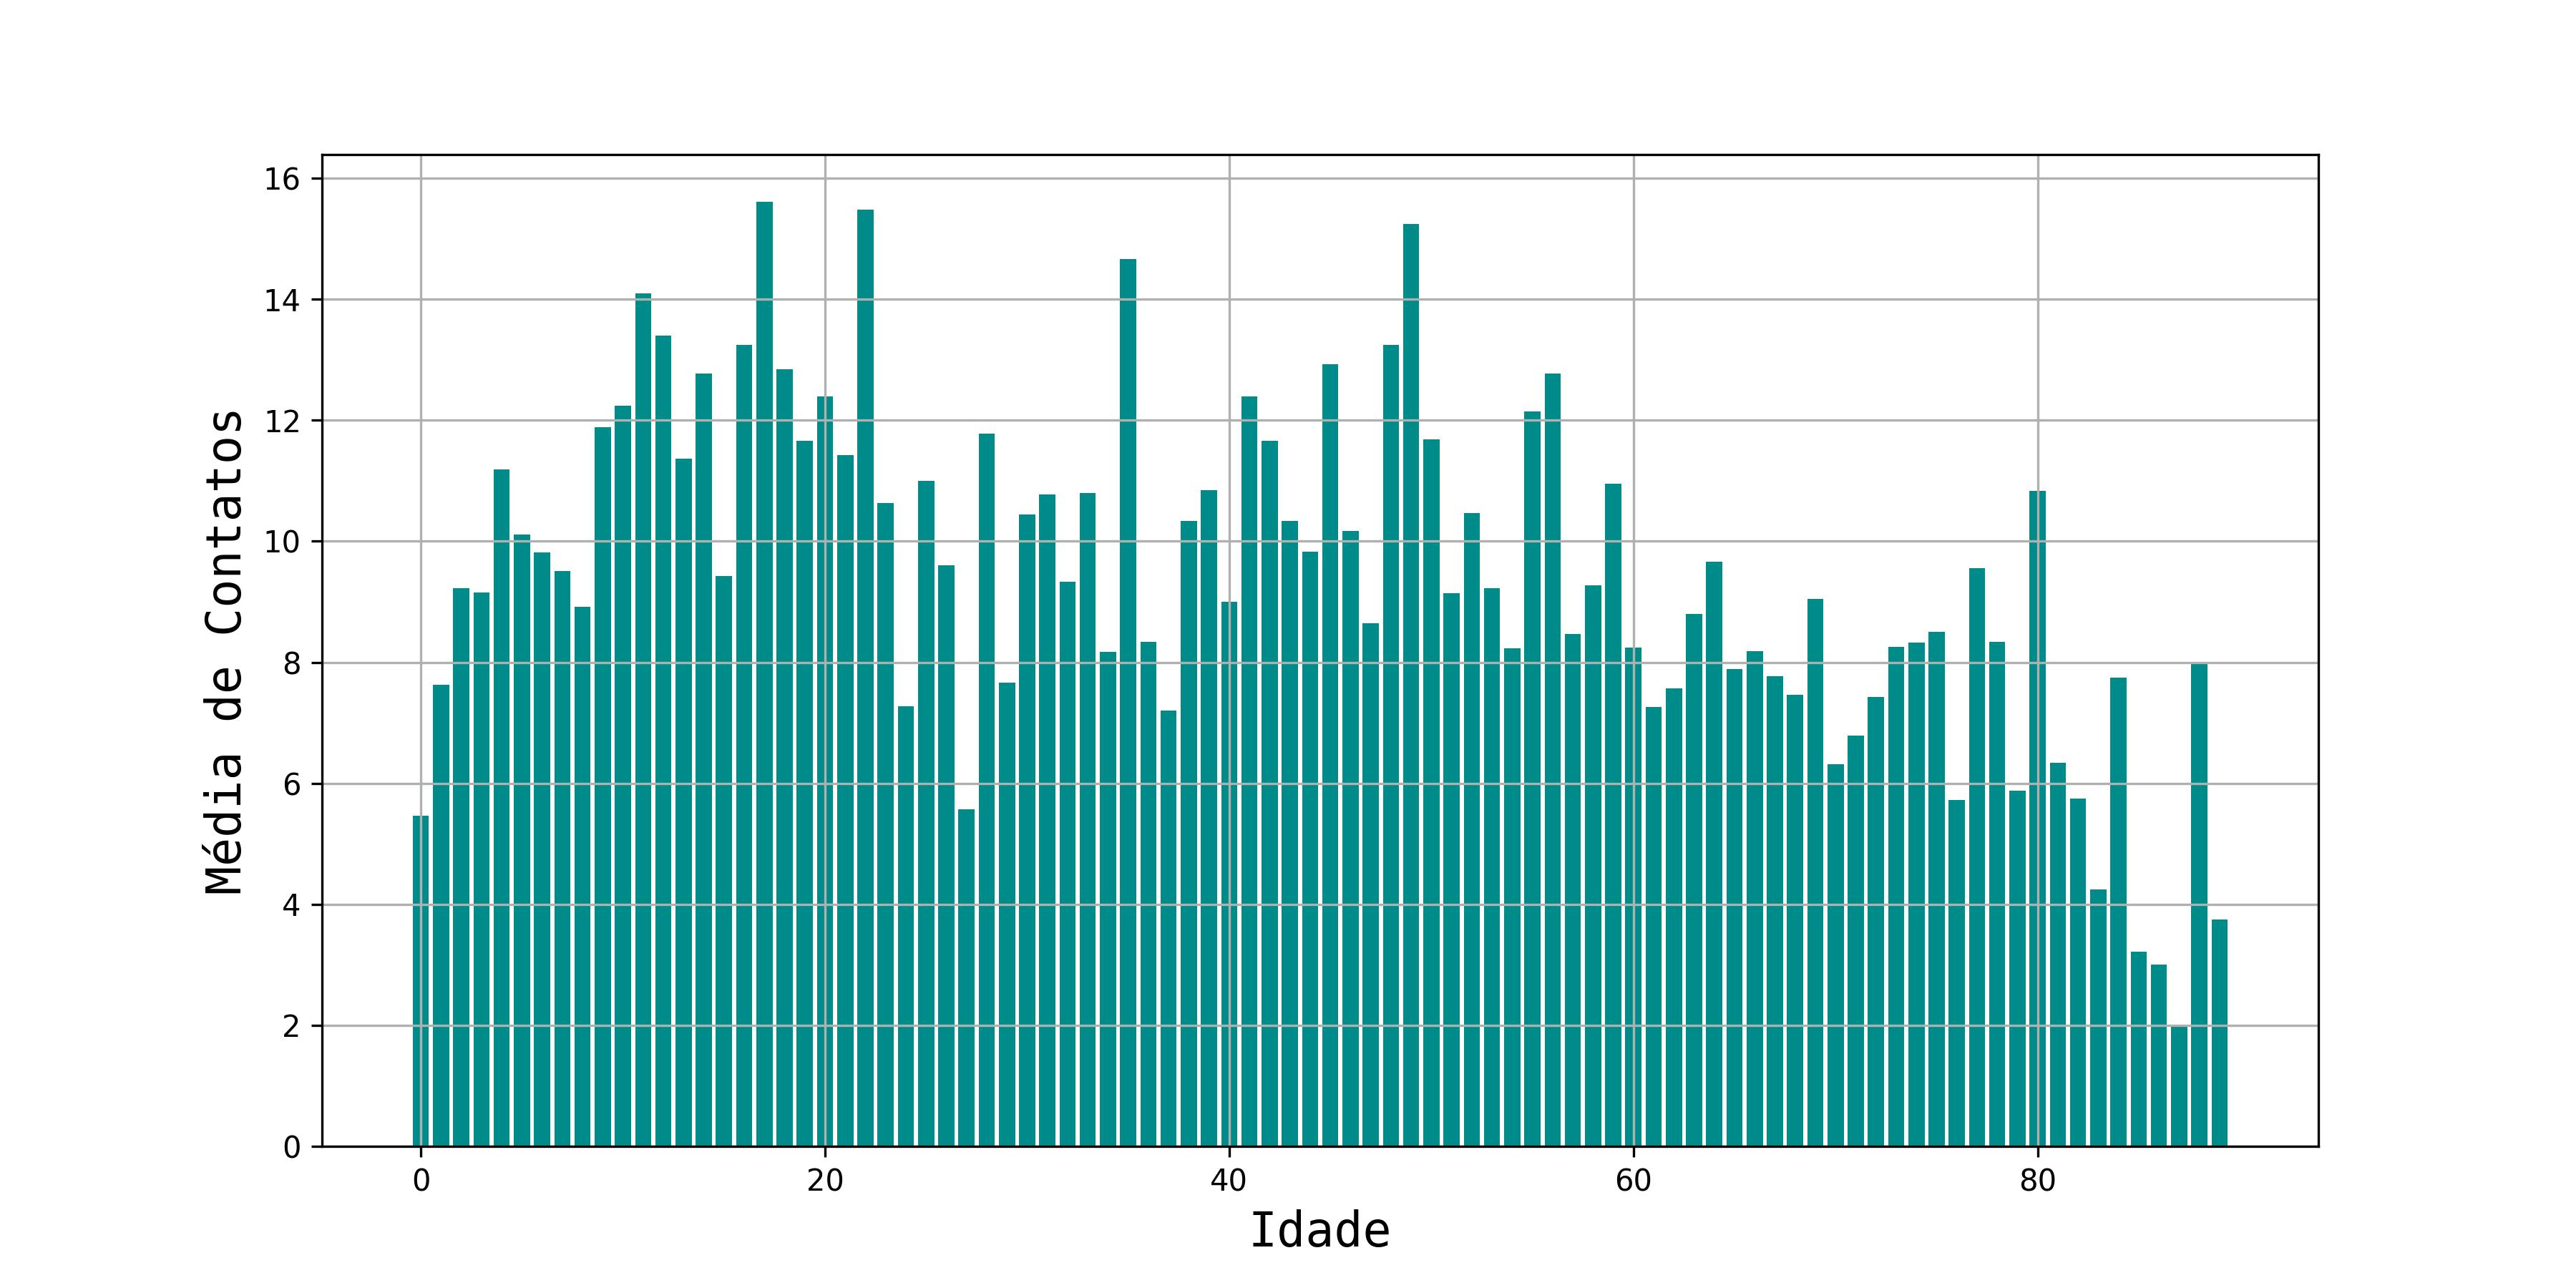
\includegraphics[scale=0.5]{./img/idade_contatos.jpg}
  \captionsetup{font=small,position=below,skip=-1pt}
   \caption*{\\Fonte: Autor.}
   \label{M_Idade}
\end{figure}

Na Figura \ref{características} observamos como os contatos são caracterizados. Quanto mais tempo nós passamos conversando com a pessoa menores as chances de acontecer algum contato físico, apesar de ser muito comum. A frequência com a qual você vê a pessoa também tem importante na probabilidade de acontecer ou não contato físico, contudo fora a primeira contato e o contado diário, praticamente a chance de haver contato físico é a mesma. A última imagem vai ao encontro dessa afirmação, percebe-se que as convivências que acontecem pela primeira vez tendem a durar em torno de minutos, enquanto que os convivências diárias podem facilmente durar horas, já em outras frequências de contatos, não parece haver uma diferenciação clara. À vista disso, há uma tendência a uma supervalorização (em questão de tempo) no contato diário pelas pessoas, há uma desvalorização na primeira vez e não há uma diferença em qualquer outra frequência.

\begin{figure}[H]
  \centering
  \captionsetup{font=normalsize,skip=1pt,singlelinecheck=on,labelsep=endash}

  \caption{Gráfico do Número de Contatos por Idade}

  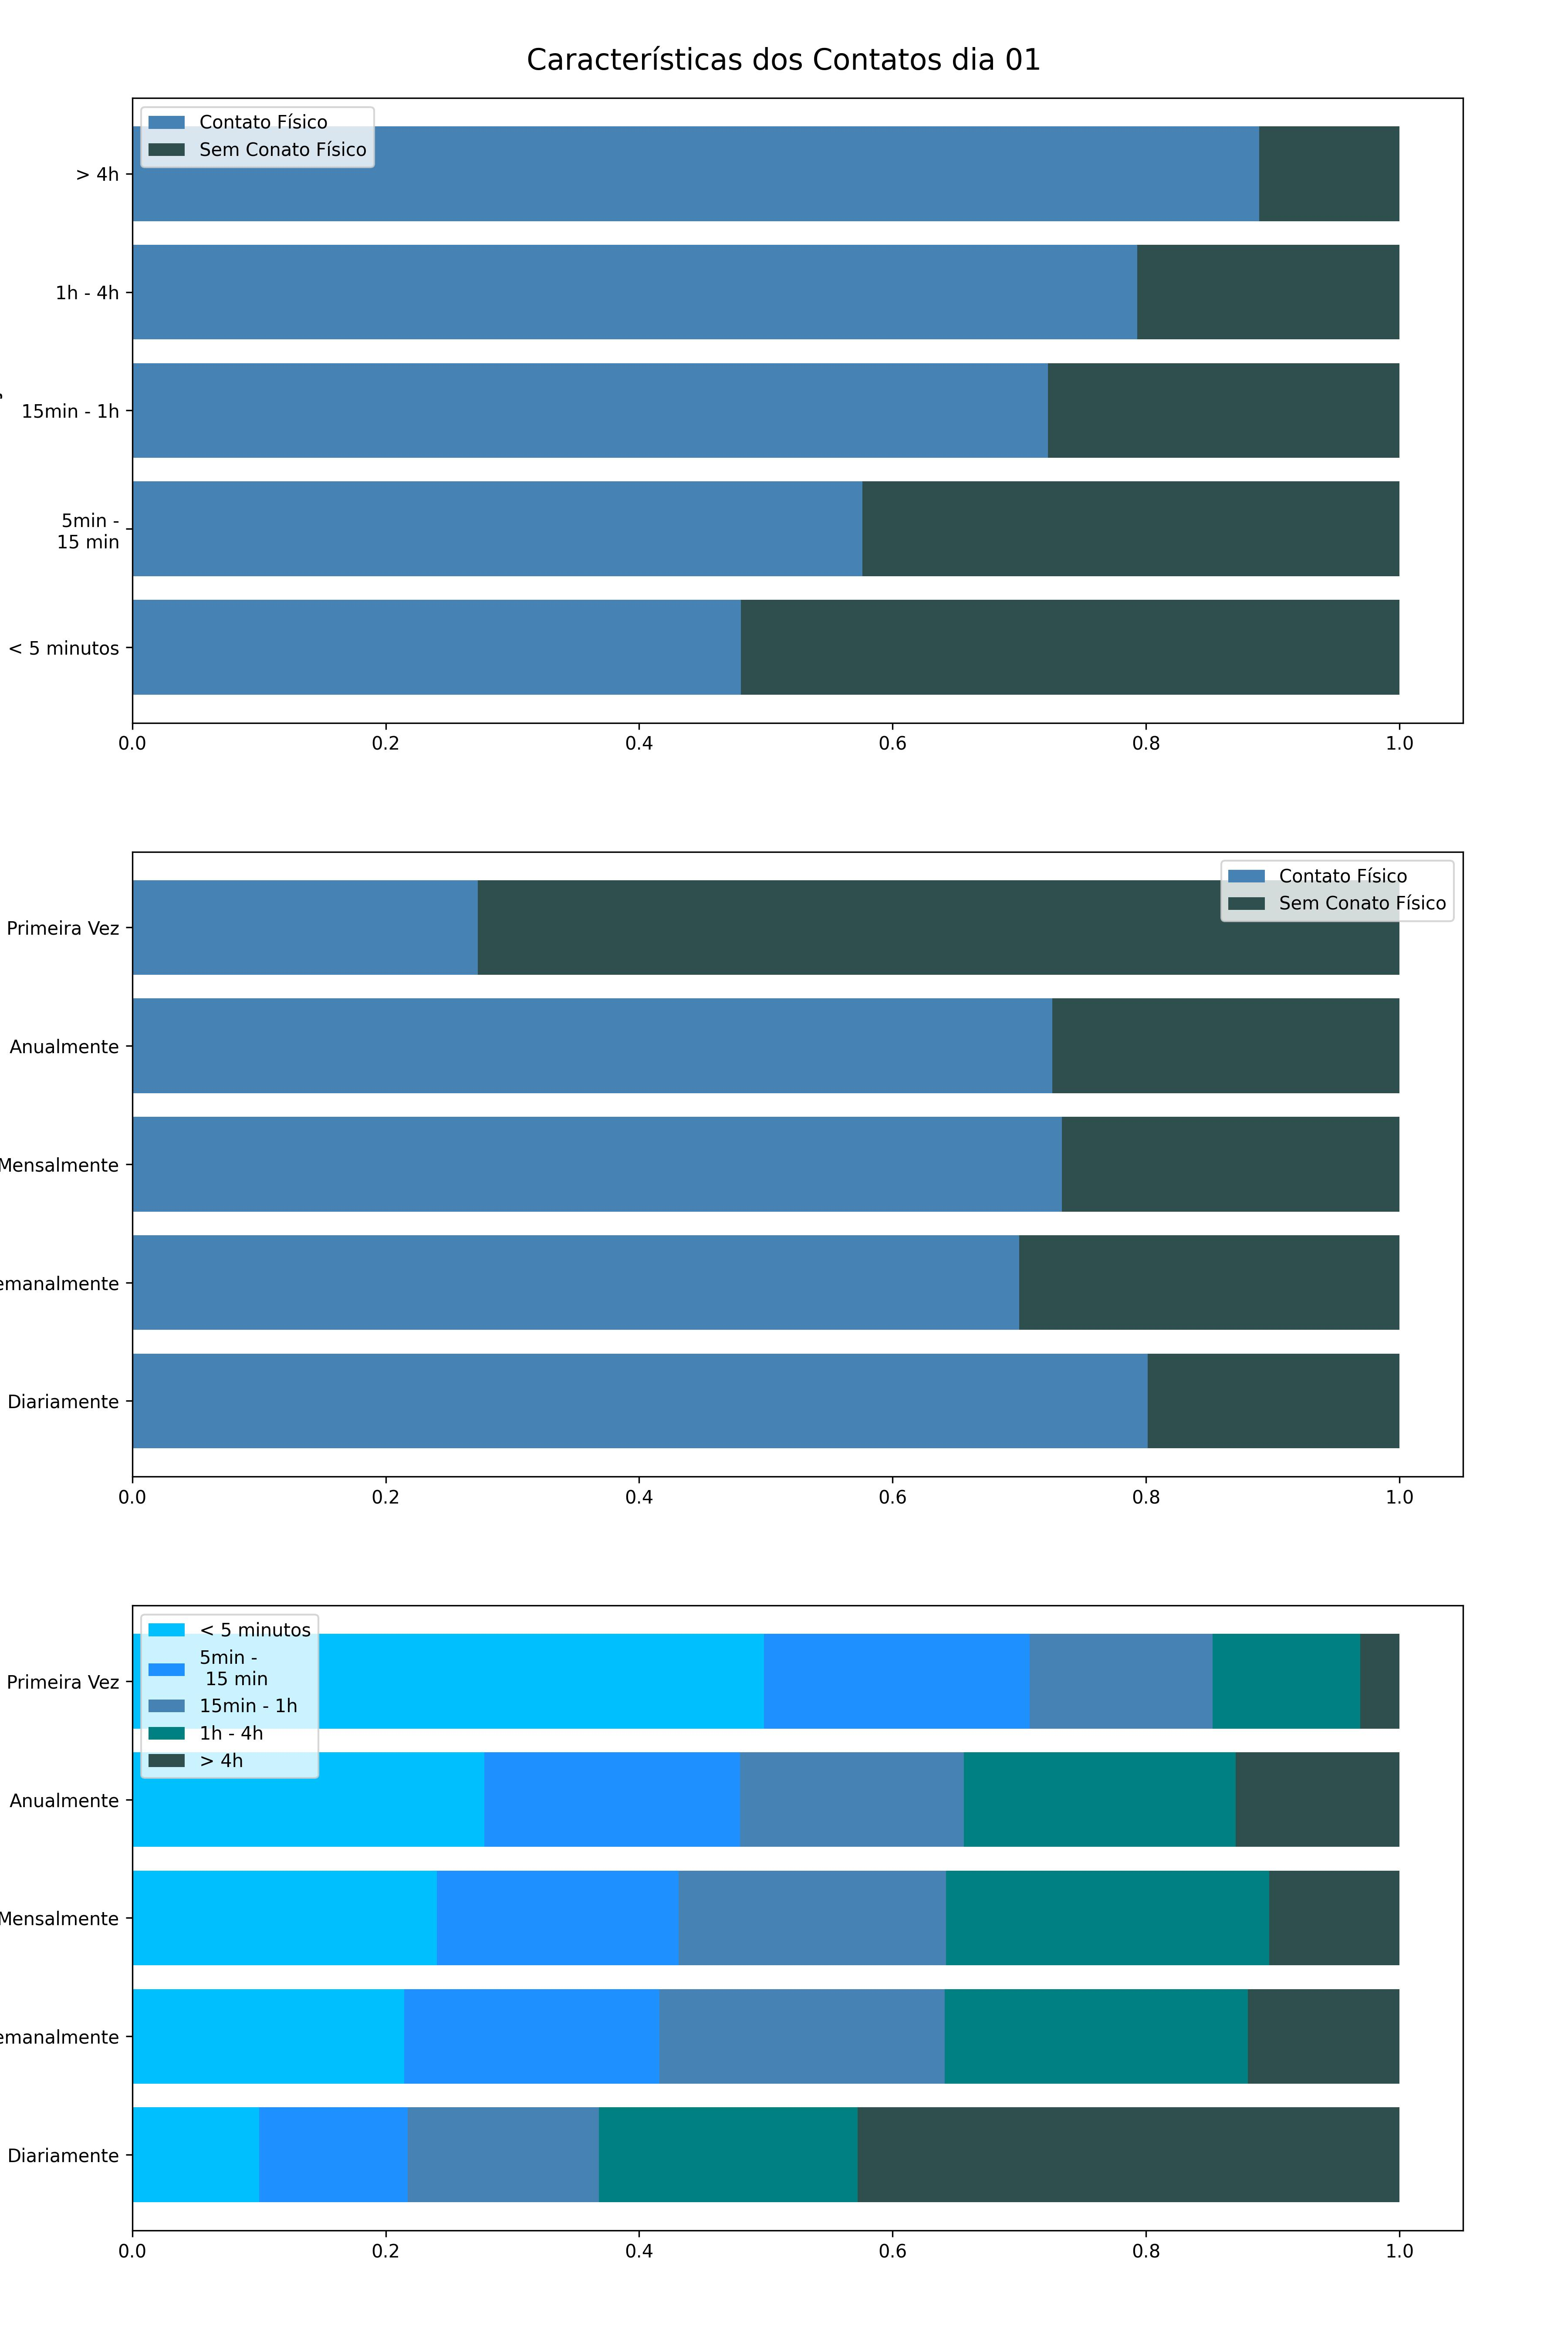
\includegraphics[scale=0.5]{./img/contatos01.jpg}
  \captionsetup{font=small,position=below,skip=-1pt}
   \caption*{\\Fonte: Autor.}
   \label{características}
\end{figure}

Apesar da grande quantidade de pessoas e contatos há um problema essencial: não há garantia de que os entrevistados se conectem em si. Por exemplo, no caso da França \cite{France} foram feitas ligações aleatórias extraída da população francesa excluindo territórios ultramarinos, assim nossa análise em rede estaria bastante limitada.

\section{Modelo de Redes}

Para evitar esse problema \cite{Manzo2020} propõe um modelo para formamos uma rede baseado nos dados franceses. A partir dos dois dias de entrevista é calculado a média de contatos por dia de cada pessoa (arredondado para cima) e utiliza o Modelo de Configuração para a formação de uma Rede Sintética. No entanto, o modelo de formação de redes gera um agrupamento médio limitado e ele é muito importante na suavização de epidemias \cite{Block2020}. Nesse sentido Manzo propõe que antes de excluirmos um dado sítio do Modelo de Configuração, passamos por cada vizinho dele e os conectamos entre si com uma probabilidade $p$. Ou seja:

\begin{enumerate}
  \item Quando um dado sítio $i$ atinge o grau requerido pelo MC selecionamos todos os vizinhos $\nu(i)$;
  \item Selecionamos dois sítios $v,n \in \nu(i)$ e conectamos com probabilidade $p$;
  \item Se ela existir os conectamos e salvamos para que ela não se repita no MC, caso contrário salvamos para que ela não se repita nesse algoritmo. Por fim também reduzimos em 1 o valor de $\kappa_v$ e $\kappa_n$ ;
  \item Fazemos 2. até testarmos todas as ligações possíveis e paramos esse algoritmo para dar continuidade ao MC.
\end{enumerate}

\begin{algorithm}

  \caption{Implementação de Manzo}\label{alg:cap}
  \begin{algorithmic}
  \Require $edges$
  \Require $\kappa$
  \Require $n\_existir$ \Comment{É necessário salvar quais ligações não vão existir.}
  \Require $p$
  \Require $i \in G(\mathpzc{N} ,\mathpzc{L})$\\

  \While{$v \in \nu(i)$}
    \While{$n \in \nu(i)$} \Comment{Nesse caso não há preferência na escolha de $n$ e $v$.}
      \If{($v \neq n$) and ($\kappa_n \neq 0$) and ($\kappa_v \neq 0$)}
          \State $r$ $\gets$ random\_number([0,1])
          \If{($r <= p$)}
            \If{($v,n$ not in $edges$) and ($v,n$ not in $n\_existir$)}
              \State $edges$.insert(($v,n$)) \Comment{Essa matriz vem do MC}
              \State $\kappa_v \gets \kappa_v - 1$
              \State $\kappa_n \gets \kappa_n - 1$
            \EndIf
          \Else
          \If{$n,v$ not in $n\_existir$}
            \State $n\_existir$.insert((v,n))
            \EndIf
          \EndIf
      \EndIf
    \EndWhile
  \EndWhile
  \end{algorithmic}

\end{algorithm}

\begin{figure}[!h]
  \centering
  \captionsetup{font=normalsize,skip=0.8pt,singlelinecheck=on,labelsep=endash}
  \caption{Ilustração do Modelo de Manzo}
  \begin{tikzpicture}[make origin horizontal center of bounding box]
    %Values
    \def\xa{2};
    \def\ya{sqrt(4-sqrt(\xa))}

    \def\xc{0.5};
    \def\yc{sqrt(4-sqrt(\xc))};

    \def\xb{0.5};
    \def\yb{sqrt(4-sqrt(\xb))};

    \def\xd{1.5};
    \def\yd{sqrt(4-sqrt(\xd))};

    \def\xe{1.3};
    \def\ye{sqrt(4-sqrt(\xe))};

    \draw[black, thick] (0,0) -- ($\xa*(1,0) + \ya*(0,1)$);

    \draw[black, thick, dotted]($\xa*(1,0) + \ya*(0,1)$) -- ($\xa*(0.5,0) + \ya*(0,0.01)$);

    
    \draw[black, thick] (0,0) -- ($\xb*(1,0) + \yb*(0,1)$);
    \draw[black, thick, dotted] ($\xb*(1,0) + \yb*(0,1)$) -- ($\xb*(1,0) + \yb*(0,1.5)$);
    \draw[black, thick, dotted] ($\xb*(1,0) + \yb*(0,1)$) -- ($\xa*(1,0) + \ya*(0,1)$);
    \draw[black, thick, dotted] ($\xb*(1,0) + \yb*(0,1)$) -- ($\xc*(1,0.5) + \yc*(0.3,0.5)$);
    \draw[black, thick, dotted] ($\xb*(1,0) + \yb*(0,1)$) -- ($\xc*(1,0.5) + \yc*(-0.3,0.5)$);

    \draw[black, thick] (0,0) -- ($\xc*(1,0) + \yc*(0,-1)$);
    \draw[black, thick, dotted] ($\xc*(1,0) + \yc*(0,-1)$) -- ($\xa*(0.7,0) + \ya*(0,0.01)$);
    \draw[black, thick, dotted] ($\xc*(1,0) + \yc*(0,-1)$) -- ($\xc*(-1.5,0) + \yc*(0,-1)$);
    

    \draw[black, thick] (0,0) -- ($\xd*(-1,0) + \yd*(0,-1)$);
    \draw[black, thick, dotted] ($\xd*(-1,0) + \yd*(0,-1)$) -- ($\xd*(-1,0) + \yd*(0,0.01)$);
    \draw[black, thick, dotted] ($\xd*(-1,0) + \yd*(0,-1)$) -- ($\xd*(-1.8,0) + \yd*(0,-1)$);

    \draw[black, thick] (0,0) -- ($\xe*(0,1) + \ye*(-1,0)$);

    % Nós

    \draw[black, fill=white, anchor=center] (0,0) circle [radius=0.25] node {3};
    \draw[black, fill=white] ($\xc*(1,0) + \yc*(0,1)$) circle [radius=0.25] node {5};
    \draw[black, fill=white] ($\xe*(0,1) + \ye*(-1,0)$) circle [radius=0.25] node {0};
    \draw[black, fill=white] ($\xd*(-1,0) + \yd*(0,-1)$) circle [radius=0.25] node {80};
    \draw[black, fill=white] ($\xb*(1,0) + \yb*(0,-1)$) circle [radius=0.25] node {32};
    \draw[black, fill=white] ($\xa*(1,0) + \ya*(0,1)$) circle [radius=0.25] node {18};
    \node at (0,3) {$p = 0$};
  \end{tikzpicture}
  \begin{tikzpicture}[make origin horizontal center of bounding box]
    %Values
    \def\xa{2};
    \def\ya{sqrt(4-sqrt(\xa))}

    \def\xc{0.5};
    \def\yc{sqrt(4-sqrt(\xc))};

    \def\xb{0.5};
    \def\yb{sqrt(4-sqrt(\xb))};

    \def\xd{1.5};
    \def\yd{sqrt(4-sqrt(\xd))};

    \def\xe{1.3};
    \def\ye{sqrt(4-sqrt(\xe))};

    \draw[black, thick] (0,0) -- ($\xa*(1,0) + \ya*(0,1)$);

    \draw[black, thick, dotted]($\xa*(1,0) + \ya*(0,1)$) -- ($\xa*(0.5,0) + \ya*(0,0.01)$);

    
    \draw[black, thick] (0,0) -- ($\xb*(1,0) + \yb*(0,1)$);
    \draw[black, thick, dotted] ($\xb*(1,0) + \yb*(0,1)$) -- ($\xb*(1,0) + \yb*(0,1.5)$);
    \draw[black, thick] ($\xb*(1,0) + \yb*(0,1)$) -- ($\xa*(1,0) + \ya*(0,1)$);
    \draw[black, thick, dotted] ($\xb*(1,0) + \yb*(0,1)$) -- ($\xc*(1,0.5) + \yc*(0.3,0.5)$);
    \draw[black, thick, dotted] ($\xb*(1,0) + \yb*(0,1)$) -- ($\xc*(1,0.5) + \yc*(-0.3,0.5)$);

    \draw[black, thick] (0,0) -- ($\xc*(1,0) + \yc*(0,-1)$);
    \draw[black, thick, dotted] ($\xc*(1,0) + \yc*(0,-1)$) -- ($\xa*(0.7,0) + \ya*(0,0.01)$);
    %\draw[black, thick, dotted] ($\xc*(1,0) + \yc*(0,-1)$) -- ($\xc*(-1.5,0) + \yc*(0,-1)$);
    

    \draw[black, thick] (0,0) -- ($\xd*(-1,0) + \yd*(0,-1)$);
    \draw[black, thick] ($\xd*(-1,0) + \yd*(0,-1)$) -- ($\xc*(1,0) + \yc*(0,-1)$);
    \draw[black, thick, dotted] ($\xd*(-1,0) + \yd*(0,-1)$) -- ($\xd*(-1.8,0) + \yd*(0,-1)$);

    \draw[black, thick] (0,0) -- ($\xe*(0,1) + \ye*(-1,0)$);

    % Nós

    \draw[black, fill=white, anchor=center] (0,0) circle [radius=0.25] node {3};
    \draw[black, fill=white] ($\xc*(1,0) + \yc*(0,1)$) circle [radius=0.25] node {5};
    \draw[black, fill=white] ($\xe*(0,1) + \ye*(-1,0)$) circle [radius=0.25] node {0};
    \draw[black, fill=white] ($\xd*(-1,0) + \yd*(0,-1)$) circle [radius=0.25] node {80};
    \draw[black, fill=white] ($\xb*(1,0) + \yb*(0,-1)$) circle [radius=0.25] node {32};
    \draw[black, fill=white] ($\xa*(1,0) + \ya*(0,1)$) circle [radius=0.25] node {18};
    \node at (0,3) {$p = 0.5$};
  \end{tikzpicture}
  \begin{tikzpicture}[make origin horizontal center of bounding box]
    %Values
    \def\xa{2};
    \def\ya{sqrt(4-sqrt(\xa))}

    \def\xc{0.5};
    \def\yc{sqrt(4-sqrt(\xc))};

    \def\xb{0.5};
    \def\yb{sqrt(4-sqrt(\xb))};

    \def\xd{1.5};
    \def\yd{sqrt(4-sqrt(\xd))};

    \def\xe{1.3};
    \def\ye{sqrt(4-sqrt(\xe))};

    \draw[black, thick] (0,0) -- ($\xa*(1,0) + \ya*(0,1)$);

    %\draw[black, thick, dotted]($\xa*(1,0) + \ya*(0,1)$) -- ($\xa*(0.5,0) + \ya*(0,0.01)$);

    
    \draw[black, thick] (0,0) -- ($\xb*(1,0) + \yb*(0,1)$);
    \draw[black, thick, dotted] ($\xb*(1,0) + \yb*(0,1)$) -- ($\xb*(1,0) + \yb*(0,1.5)$);
    \draw[black, thick] ($\xb*(1,0) + \yb*(0,1)$) -- ($\xa*(1,0) + \ya*(0,1)$);
    \draw[black, thick, dotted] ($\xb*(1,0) + \yb*(0,1)$) -- ($\xc*(1,0.5) + \yc*(0.3,0.5)$);
    %\draw[black, thick, dotted] ($\xb*(1,0) + \yb*(0,1)$) -- ($\xc*(1,0.5) + \yc*(-0.3,0.5)$);

    \draw[black, thick] (0,0) -- ($\xc*(1,0) + \yc*(0,-1)$);
    %\draw[black, thick, dotted] ($\xc*(1,0) + \yc*(0,-1)$) -- ($\xa*(0.7,0) + \ya*(0,0.01)$);
    %\draw[black, thick, dotted] ($\xc*(1,0) + \yc*(0,-1)$) -- ($\xc*(-1.5,0) + \yc*(0,-1)$);
    

    \draw[black, thick] (0,0) -- ($\xd*(-1,0) + \yd*(0,-1)$);
    \draw[black, thick] ($\xd*(-1,0) + \yd*(0,-1)$) -- ($\xc*(1,0) + \yc*(0,-1)$);
    \draw[black, thick] ($\xd*(-1,0) + \yd*(0,-1)$) -- ($\xb*(1,0) + \yb*(0,1)$);
    \draw[black, thick] ($\xb*(1,0) + \yb*(0,-1)$) -- ($\xa*(1,0) + \ya*(0,1)$);

    \draw[black, thick] (0,0) -- ($\xe*(0,1) + \ye*(-1,0)$);

    % Nós

    \draw[black, fill=white, anchor=center] (0,0) circle [radius=0.25] node {3};
    \draw[black, fill=white] ($\xc*(1,0) + \yc*(0,1)$) circle [radius=0.25] node {5};
    \draw[black, fill=white] ($\xe*(0,1) + \ye*(-1,0)$) circle [radius=0.25] node {0};
    \draw[black, fill=white] ($\xd*(-1,0) + \yd*(0,-1)$) circle [radius=0.25] node {80};
    \draw[black, fill=white] ($\xb*(1,0) + \yb*(0,-1)$) circle [radius=0.25] node {32};
    \draw[black, fill=white] ($\xa*(1,0) + \ya*(0,1)$) circle [radius=0.25] node {18};
    \node at (0,3) {$p = 1$};
  \end{tikzpicture}
  \captionsetup{font=small}
  \caption{Funcionamento do Modelo de Configuração, escolhemos dois sítios $i$ e $j$ aleatoriamente e os conectamos. O Algoritmo pode gerar várias topologias de redes, porém ainda limitadas pelas quantidades $\{k_i\}$ de graus impostas pelo MC.\\ Fonte: Elaborado pelo autor}
  \label{img:MC_P}
\end{figure}

O Modelo é mostrado na Figura \ref{img:MC_P}, na qual mostramos o estágio quando encontramos um dado sítio que atinge o grau especificado. Assim como nos modelos de formação de rede existem várias redes que podem ser formadas dada uma probabilidade $p$. Outrossim, se o sítio já tiver atingido o grau requerido pelo MC, então ele não precisa entrar nesse algoritmo. A partir desse modelo o autor consegue os seguintes resultados mostrados na Tabela \ref{table:Manzo} e os meus estão na Tabela \ref{table:Miguel}.

\begin{table}[H]
  \centering
  \captionsetup{margin={9pt,14pt},font=normalsize,skip=0.5pt,labelsep=endash}

  \caption{Tabela do resultado de Manzo}
  \hspace*{-\leftmargin}\begin{tabular}{lccccccc}

    \hline

    \multicolumn{1}{l|}{ \textbf{\shortstack{Probabi\\-lidade}}} & 
    \multicolumn{1}{c|}{\textbf{\shortstack{Grau \\ Médio}}}  & 
    \multicolumn{1}{c|}{\textbf{\shortstack{Grau \\ Mediano}}} &
    \multicolumn{1}{c|}{\textbf{\shortstack{Desvio \\ Padrão \\ Grau}}} &
    \multicolumn{1}{c|}{\textbf{\shortstack{Agrupa-\\mento \\ Médio}}} & 
    \multicolumn{1}{c|}{\textbf{\shortstack{Corr \\ Agrup-\\ Grau}}} & 
    \multicolumn{1}{c|}{\textbf{\shortstack{Menor \\ Caminho \\ Médio}}} & 
    \multicolumn{1}{c}{{\shortstack{\textbf{Diâmetro}}}}     \\

    \hline\\
    \rowcolor{Gray}
p = 0         & 9.72 (0.00) & 8 (0.00)     & 6.56 (0.00)        & 0.01 (0.00)       & -0.06 (0.01)                  & 3.47 (0.00)         & 6 (0.00)     \\
  p = 0.5       & 9.72 (0.00) & 8 (0.00)     & 6.56 (0.00)        & 0.43 (0.00)       & -0.62 (0.01)                  & 4.38 (0.03)         & 7.45 (0.5)   \\
  \rowcolor{Gray}
  p = 1.0       & 9.72 (0.00) & 8 (0.00)     & 6.56 (0.00)        & 0.57 (0.01)       & -0.56 (0.01)                  & 5.52 (0.09)         & 10.10 (0.59)

  
\end{tabular}

  \captionsetup{margin={10pt,10pt},font=small,skip=0pt,position=below}

  \caption{Nessa tabela são apresentados resultados advindos do autor para a rede francesa feitas em 100 simulações de redes. Apresentando as características da rede e em parêntese o erro associado a cada valor. \\Fonte: Elaborada pelo autor.}
\label{table:Manzo}
\end{table}

Os valores com probabilidade $p = 0$ batem perfeitamente com os resultados do autor, os outros valores se aproximam bastante do que aparece no artigo, porém ainda na mesma faixa de erro. Podemos ver que o Grau permanece o mesmo para que seja respeitado o MC já o agrupamento aumenta bastante com o incremento de $p$ chegando a seu valor máximo em $0.56$ que é limitado pelo MC.

\begin{table}[H]
  \centering
  \captionsetup{margin={9pt,14pt},font=normalsize,skip=0.5pt,labelsep=endash}

  \caption{Tabela do meu resultado.}
  \hspace*{-\leftmargin}\begin{tabular}{lccccccc}

    \hline

    \multicolumn{1}{l|}{ \textbf{\shortstack{Probabi\\-lidade}}} & 
    \multicolumn{1}{c|}{\textbf{\shortstack{Grau \\ Médio}}}  & 
    \multicolumn{1}{c|}{\textbf{\shortstack{Grau \\ Mediano}}} &
    \multicolumn{1}{c|}{\textbf{\shortstack{Desvio \\ Padrão \\ Grau}}} &
    \multicolumn{1}{c|}{\textbf{\shortstack{Agrupa-\\mento \\ Médio}}} & 
    \multicolumn{1}{c|}{\textbf{\shortstack{Corr \\ Agrup-\\ Grau}}} & 
    \multicolumn{1}{c|}{\textbf{\shortstack{Menor \\ Caminho \\ Médio}}} & 
    \multicolumn{1}{c}{{\shortstack{\textbf{Diâmetro}}}}     \\

    \hline\\ \rowcolor{Gray}
    p = 0 & 9.72(0.00) & 8.00(0.00) & 6.56(0.00) & 0.01(0.00) & -0.06(0.01) & 3.47(0.00) & 6.00(0.03)  \\
p = 0.5                             & 9.72(0.00)                      & 8.00(0.00)   & 6.56(0.00)         & 0.43(0.01)        & -0.62(0.01)                   & 4.37(0.05)          & 7.46(0.50)  \\
p = 1.0                             & 9.72(0.00)                      & 8.00(0.00)   & 6.56(0.00)         & 0.56(0.01)        & -0.57(0.01)                   & 5.62(0.11)          & 10.39(0.66)

  
\end{tabular}

  \captionsetup{margin={10pt,10pt},font=small,skip=0pt,position=below}

  \caption{Nessa tabela são apresentados resultados advindos do meu código na qual foram feitas 1000 simulações de redes para a rede francesa que se aproximam bastante do apresentado no artigo junto com os desvios padrões entre parênteses. Os que não bateram certo estão na faixa de erro mostrada anteriormente. \\Fonte: Elaborada pelo autor.}
\label{table:Miguel}
\end{table}



\newpage
\mycomment{


\begin{table}[h]
  \centering
\captionsetup{margin={9pt,14pt},font=normalsize,skip=0.5pt,labelsep=endash}
\caption{Distribui\c c\~ao dos documentos analisados por programa de p\'os-gradua\c c\~ao}
        \begin{tabular}{l|c|c|c}
           %\specialrule{1pt}{0pt}{0pt}
%    \multirow{2}{*}{\textbf{Programas de p\'os-gradua\c{c}\~ao~~~~~~~}}
    & \multicolumn{2}{c|}{\textbf{Categoria}}  &  \multirow{2}{*}{\textbf{~Total~}} \\
            \cline{2-3}
             & \textbf{~~~~~Teses~~~~~} & \textbf{Disserta\c{c}\~oes} &  \\
            \hline
            Cirurgia  & 1 & 1 & 2 \\
            Enfermagem & 4 &4 & 8 \\
            Engenharia Civil & 2 & 8 & 10 \\
            Farmacologia & 8 & 6 & 14 \\
            F\'isica & 3 & 6 & 9 \\
            Qu\'imica Inorg\^anica & 4 &1 & 5 \\
            {\bf Total}   & {\bf 22} & {\bf 26} & {\bf 48} \vspace{-0.6mm}\\ \bottomrule[1pt]
        \end{tabular}
\captionsetup{margin={10pt,10pt},font=small,skip=0pt,position=below}
\caption*{Fonte: Elaborada pelo autor.}
\end{table}

\begin{figure}[h]
\centering
\captionsetup{font=normalsize,skip=1pt,singlelinecheck=on,labelsep=endash}
\caption{Figura teste}

\includegraphics[scale=0.5]{ufc.jpg}
\captionsetup{font=small,position=below,skip=-1pt}
 \caption*{Fonte: Lara e Smit.}
 \label{fig1}
\end{figure}

\vskip2cm


\begin{grafico}[h]
\centering
\captionsetup{font=normalsize,skip=0.8pt,singlelinecheck=on,labelsep=endash}
\caption{Grafico de teste}

\includegraphics[scale=0.5]{ufc.jpg}
\vspace{-0,15cm}
\captionsetup{font=small}
  \caption*{Fonte: Elaborado pelo autor.}
  \label{graf1}
\end{grafico}
\newpage
\begin{grafico}[h]
\centering
\captionsetup{font=normalsize,skip=0.8pt,singlelinecheck=on,labelsep=endash}
\caption{Grafico de teste2}

\includegraphics[scale=0.5]{ufc.jpg}
\vspace{-0,15cm}
\captionsetup{font=small}
  \caption*{Fonte: Elaborado pelo autor.}
  \label{graf2}
\end{grafico}

}

\section{Modelo de Infecção}

Como discutido anteriormente a pandemia do COVID-19 teve bastante impacto na sociedade e um deles foi no aumento nos estudos de modelos epidemiológicos, criando modelos mais robustos \cite{Xiang2021} considerando mais do que apenas infectados e suscetíveis. Além disso esses modelos estão em formato de equações diferencias e isso tem implicações no modelagem na qual é considerado que todos os indivíduos conseguem propagar a doença para qualquer outro indivíduo. Além disso, nesse formato de modelagem estamos estudando o nosso sistema de forma macroscópica e quando se tenta modelar utilizando redes estamos tentando estudar de forma microscópica, portanto a escolha de qual modelo é essencial e como ele se comporta de forma microscópica é essencial. Então qual modelo iremos escolher?

Para responder essa pergunta temos que entender qual o propósito de vacinas. As vacinas têm como principal função reduzir a propagação da enfermidade e impedir que os indivíduos que por ventura se contaminem não apresentem os efeitos mais graves da doença. Por fim não só é considerado o fator humano mas também econômico como é o caso da superlotação de hospitais \cite{French2021}. Nesse sentido não é apenas o espaço físico da UTI ou Hospital que está sendo utilizado, mas também de remédios, equipes de saúde e suprimentos, que poderiam estar sendo alocados em outras localidades e também prejudica pessoas que precisariam do espaço para outros problemas. À vista disso, usaremos como métricas para serem minimizadas são o número básico de reprodução $R_0$, número de mortos $M$ e número de Hospitalizações $M_H$.

Assim sendo, o modelo de contágio a ser utilizado é o chamado SEIHARD como base para nossa primeira aproximação. Nele temos os sítios que podem se apresentar como Suscetíveis, Expostos, Infectados Sintomáticos, Hospitalizados, Infectados Assintomáticos, Recuperados e Mortos. Esse modelo é uma adaptação de \cite{Eikenberry2020} e \cite{SEIHR}, podemos definir cada estágio da seguinte forma:

\begin{itemize}
  \item \textbf{Suscetível (S)}: é o sítio que tem conexões na rede e não foi infectado pelo vírus ainda;
  \item \textbf{Exposto (E)}: um sítio é considerado exposto quando ele estava no estágio S e foi contaminado por alguém no estágio E ou A. Esse estágio é para representar os indivíduos que estão na fase de encubação do vírus, isso faz com que eles possam contaminar as outros indivíduos por não saberem que tem a doença;
  \item \textbf{Infectado Sintomático (I)}: um sítio nesse estágio está infectado, porém ele não pode infectar outras pessoas. Fazendo isso estamos tentando emular uma pessoa que está sentindo os sintomas e por isso não teria mais contato com outras pessoas;
  \item \textbf{Hospitalizado (H)}: nele o nó continua sem a capacidade de contaminar outros nós. Nessa primeira aproximação estamos considerando que podemos ter qualquer quantidade de sítios hospitalizados, o que não é verdade por isso a posteriori iremos atualizar essa parte para melhorar o modelo;
  \item \textbf{Infectado Assintomático (A)}: a diferença desse estágio para o I é o fato de que ele pode infectar outras pessoas. Isso se deve ao fato de que se ele é assintomático então não tem conhecimento da doença por não sentir nenhum sintoma, portanto ele continua tendo as suas ligações e também não tem risco de morte ou necessidade de ser hospitalizado;
  \item \textbf{Recuperado (R)}: caso o nó não morra ele será considerado Recuperado.
  \item \textbf{Morto (D)}: Por fim, nesse o sítio perde todas as conexões e é nele que será contabilizado quantas pessoas morreram para utilizarmos como métrica de minimização.
\end{itemize}

\begin{figure}[H]
  \centering
  \captionsetup{font=normalsize,skip=0.8pt,singlelinecheck=on,labelsep=endash}
  \caption{Ilustração do Modelo SEIHARD}
  \begin{tikzpicture}

    \draw[->] (2,2.5) -- node[above] {\small $\epsilon_s \frac{E}{N} + \epsilon_a\frac{I}{N}$} (3.9,2.5) ;
    \draw[->] (6,2.8) -- node[above,rotate=32]{$(1 - \alpha^i)\sigma$} (7.9,4);
    \draw[->] (6,2) -- node[below,rotate=-32]{$\alpha^i\sigma$} (7.9,1);
    \draw[->] (10,1) -- node[above] {$\psi^i\phi$} (11.98,1);
    \draw[->] (13.5,0.5) -- node[above,rotate=-38] {$\tau^i\delta$} (15,-0.9);
    \draw[->] (12.5,0.9) -- node[below,rotate=45] {$(1 - \tau^i)\gamma_H$} (11,-0.9);
    \draw[->] (9,1) -- node[below,rotate=-38] {$(1 - \psi^i)\gamma_I$} (10.8,-0.9);
    \draw[->, dashed] (10,4) parabola (10.9,-0.8);
    \node[draw,fill = white,draw = white] at (10.5,2.8) {$\gamma_A$};
    
    \draw[rounded corners,drop shadow, fill=ninfect,draw=border, ultra thick] (0,2) rectangle (2,3)node[pos=.5,text= white,font=\fontsize{20}{20}\selectfont]  {S};
    
    \draw[rounded corners,drop shadow, fill=infect,draw=border, ultra thick](4, 2) rectangle (6,3) node[pos=.5,text= white,font=\fontsize{20}
    {20}\selectfont]  {E};
    
    \draw[rounded corners,drop shadow, fill=infect,draw=border, ultra thick](8, 3.5) rectangle (10,4.5) node[pos=.5,text= white,font=\fontsize{20}
    {20}\selectfont]  {A};
    
    \draw[rounded corners,drop shadow, fill=ninteract,draw=border, ultra thick](8, 0.5) rectangle (10,1.5) node[pos=.5,text= white,font=\fontsize{20}
    {20}\selectfont]  {I};
    
    \draw[rounded corners,drop shadow, fill=ninteract,draw=border, ultra thick](12, 0.5) rectangle (14,1.5) node[pos=.5,text= white,font=\fontsize{20}
    {20}\selectfont]  {H};
    
    \draw[rounded corners,drop shadow, fill=ninteract,draw=border, ultra thick](14, -1) rectangle (16,-2) node[pos=.5,text= white,font=\fontsize{20}
    {20}\selectfont]  {D};
    
    \draw[rounded corners,drop shadow, fill=ninteract,draw=border, ultra thick](10, -1) rectangle (12,-2) node[pos=.5,text= white,font=\fontsize{20}
    {20}\selectfont]  {R};
    
    
    
  \end{tikzpicture}
  \captionsetup{font=small}
  \caption{Esquematização do Modelo SEIHARD de contágio. Os blocos em vermelho significam quem pode contaminar outros, os blocos em azul escuro quem não é infectado e em azul claro quem está isolado da rede.}
  \label{img:Contagio}
\end{figure}



\begin{table}[H]
  \caption{Tabela de parâmetros do modelo.}
  \begin{tabular}{cll}
  Parâmetro & Definição & Valor [Referência] \\
  \hline
  \rowcolor{Gray}
  $\epsilon_s$ & Proporção de Infecção de Sintomáticos & 0.5 $day^{-1}$\\
  $\epsilon_a$ & Proporção de Infecção de Assintomáticos& 0.41 $day^{-1}$\\ 
  \rowcolor{Gray}
  $\alpha^i$   & Fração de Infectados que tornarão-se Sintomáticos & Tabela \ref{alpha} \cite{Jung2020}\\
  $\sigma$     & Transição exposta a infecções& 1/5.1 day$^{-1}$\\
  \rowcolor{Gray}
  $\gamma_A$   & Taxa de Recuperação de Assintomáticos& $1/7 day^{-1}$\\
  $\gamma_H$   & Taxa de Recuperação de Hospitalizados& $1/14 day^{-1}$\\
  \rowcolor{Gray}
  $\gamma_I$   & Taxa de Recuperação de Sintomáticos & $1/7 day^{-1}$\\
  $\phi$     & Taxa de Hospitalização & 0.025 $day^{-1}$\\
  \rowcolor{Gray}
  $\psi^i$   & Probabilidade de Hospitalização & Tabela \ref{psi}\\
  $\delta$   & Taxa de Mortalidade & 0.015 $day^{-1}$\\
  \rowcolor{Gray}
  $\tau^i$   & Probabilidade de Morte & Tabela \ref{tau}
  \end{tabular}

  \caption*{Fonte: Elaborada pelo autor.}

\end{table}


\begin{table}[H]
  \centering
  \begin{tabular}{llllll}
  Faixa & 0 - 20 & 20 - 30 & 30 - 50 & 50 - 70 & \textgreater{}= 70 \\
  \hline
  Valor & 29,1\% & 37,4\%  & 41.68\% & 39.4\%  & 31.3\%            
  \end{tabular}

  \caption{Nessa tabela são apresentados os valores de $\alpha^i$, que é a probabilidade de se tornar sintomático pela idade. \\Fonte: Elaborada pelo autor.}

  \label{alpha}

\end{table}

\begin{table}[H]
  \centering
  \begin{tabular}{llllll}
  Faixa & 0 - 20 & 20 - 30 & 30 - 50 & 50 - 70 & \textgreater{}= 70 \\
  \hline
  Valor & 0.408\% & 1.04\%  & 3.89\% & 9.98
  \%& 17.5\%
  \end{tabular}

  \caption{Nessa tabela são apresentados os valores de $\psi^i$, que é a probabilidade de um infectado ser hospitalizado. \\Fonte: Elaborada pelo autor.}

  \label{psi}

\end{table}

\begin{table}[H]
  \centering
  \begin{tabular}{llllll}
  Faixa & 0 - 20 & 20 - 30 & 30 - 50 & 50 - 70 & \textgreater{}= 70 \\
  \hline
  Valor & 1.04\% & 1.33\%  & 1.38\% & 7.6\%  & 24\%            
  \end{tabular}

  \caption{Nessa tabela são apresentados os valores de $\tau^i$, que é a probabilidade de um hospitalizado morrer. Esses dados foram coletados a partir do Open Data SUS do ano de 2020. \\Fonte: Elaborada pelo autor.}

  \label{tau}

\end{table}